\subsubsection{Multiplicative decomposition and density transformation}
The key idea of the kinematics of the growth model is the multiplicative decomposition of deformation gradient $\bF$ into an elastic part $\bF_\rme$ and a growth part $\bF_\rmg$. Based on the work in \cite{Himpel, Goktepe2}, an intermediate configuration $B_\rmg$ is introduced between the reference configuration $B_0$ and the current configuration $B_\rmt$. As shown in Figure \ref{fig:decomposition},
$\phi$ is the mapping from $B_0$ to $B_\rmt$, and the deformation gradient $\bF$ is defined in regular way as $\bF = \nabla_\bX \phi$. We assume there exists a decomposition:
\begin{equation} \label{eq:decomposition}
\bF = \bF_\rme \cdot \bF_\rmg
\end{equation}

\begin{figure}[H]
	\centering
	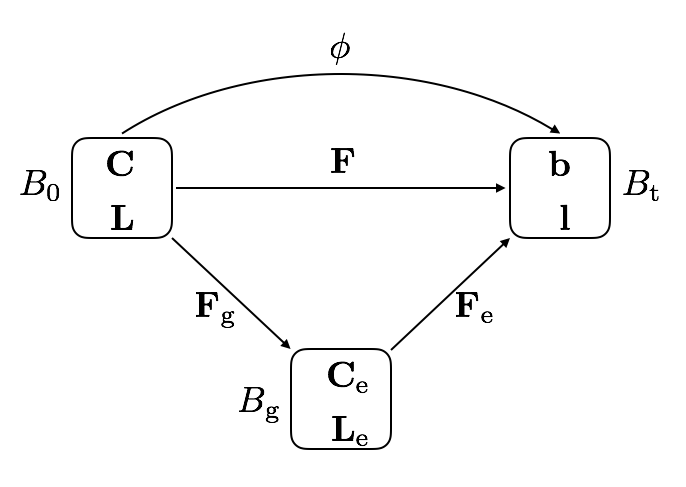
\includegraphics[width=0.45\textwidth]{./figs/decomposition.png}
	\caption{The intermediate configuration and the decomposition of deformation gradient}
	\label{fig:decomposition}
\end{figure}

Similarly, the right Cauchy-Green tensor $\bC$, velocity gradient $\bl$, Piola-Kirchhoff stress $\bold{P}$ and the second Piola-Kirchhoff (PK2) stress $\bS$ can be decomposed into elastic and growth parts as well.  Because of the growth of mass, the mapping $\phi$ is ``one-to-one'', but not ``onto''. Therefore the intermediate configuration is incompatible \cite{Cowin}.

Next we consider the density expressions in different configurations, which is the basis of the balance equations. Let $\rho_0$ denote the density in the reference configuration, $\rho_\rmt$ and $\rho_\rmg$ denote its counterparts in the spatial configuration and the intermediate configuration, respectively. Similarly, define the volume of a material particle in the reference,  spatial and intermediate configurations as $dV$, $dv$ and $dV_\rmg$, respectively. In analogy to $J = \mathrm{det}\bF$, define the Jacobians $J_\rme = \mathrm{det}\bFe$ and $J_\rmg = \mathrm{det}\bFg$. The transformations of the volumes become:
\begin{equation} \label{eq:volume}
dv = JdV, \quad dV_\rmg = J_\rmg dV, \quad dv = J_\rme dV_\rmg
\end{equation}
and
\begin{equation} \label{eq:det}
J = J_\rme J_\rmg
\end{equation}

Based on the definitions, we have the following density transformations:
\begin{equation} \label{eq:mass}
\rho_\rmg dV_\rmg = \rho_\rmt dv, \quad \rho_\rmg = J_\rme\rho_\rmt
\end{equation}

\subsubsection{Balance laws}
The local form of the balance of mass balances the rate of change of the grown density ${\bar{\rho}}_0$ with 
a possible mass flux $\bold{R}$ and a possible mass source $R_0$,
\begin{equation}
\dot{\bar{\rho}}_0 = \nabla_\bold{X} \cdot \bold{R} + R_0
\end{equation}
where the grown density is defined in the reference configuration and can be expressed as $\grho = J\rho_\rmt = J_\rmg \rho_\rmg$. From a microscopic point of view, the mass flux can be related with cell migration and the mass source can be associated to cell proliferation, hyperplasia, hypertrophy, mitosis, necrosis, and apoptosis \cite{Menzel}.

The linear momentum balance, compared to the original form, contains an additional term due to the density change:
\begin{equation} \label{eq:momentum}
\dot{\bar{\rho}}_0 \bv + {\bar{\rho}}_0\dot{\bv} = \nabla_\bX \cdot \bold{P} + {\bar{\rho}}_0\bold{b}
\end{equation}

The balance of entropy is built on the assumption that the temperature $\theta$ remains constant, which is reasonable for living biological tissues. The local form of the dissipation inequality is written as:
\begin{equation} \label{eq:entropy}
\grho \mathcal{D}= \bold{P} : \dot{\bF} - \grho \dot \Psi  - \theta(\nabla_\bX \cdot \bS - S_0) \geq 0
\end{equation}
where $\Psi$ is the free energy per unit mass and $\bS$ and $S_0$ are the extra entropy flux and source that are necessary to satisfy the second law of thermodynamics.

\subsubsection{Constitutive equations of growth}
In general, the constitutive equations for finite growth consists of three components: (i) the definition of the stress, which can be derived as conjugate counterpart of the deformation tensors; (ii) the definition of the growth tensor $\bF_\rmg$, which can be either compressible or incompressible, either isotropic or anisotropic, based on the microstructure of the modeling object; (iii) the definition of a internal variable to evaluate the growth process and a set of evolution equations to characterize it. Assume an isotropic hyperelastic model with the Helmholtz free energy $\phi(\bC, \bF_\rmg)$ (an extension to anisotropic hyperelastic model is straightforward, but is not of our interest in this project), the PK2 stress and Kirchhoff stress can be evaluated as:
\begin{subequations} \label{eq:stress}
\begin{equation}
\bS = 2\frac{\partial \Psi}{\partial \bC} = 2\frac{\partial \Psi}{\partial \bC_\rme} : \frac{\partial \bC_\rme}{\partial \bC} = \bF_{\rmg}^{-1} \cdot \bS_\rme \cdot \bF_\rmg^{-T}
\end{equation}
\begin{equation}
\boldsymbol{\tau} = \bF \cdot \bS \cdot \bF^T = \bF_\rme \cdot \bS_\rme \cdot \bF_\rme^T
\end{equation}
\end{subequations}
where $\bS_\rme$ denotes the elastic part of $\bS$. The constitutive moduli $\bold{L}$ and $\bold{e}$ read:
\begin{subequations} \label{eq:moduli}
\begin{equation}
\bold{L} = 2\frac{d\bS(\bF, \bF_\rmg)}{d\bC}
\end{equation}
\begin{equation}
\bold{e} = (\bF \overline\otimes \bF) : \bL : (\bF^T \overline\otimes \bF^T)
\end{equation}
\end{subequations}
It can be seem immediately from Equations \ref{eq:stress} and \ref{eq:moduli} that both the stress and its constitutive modulus differ from their usual form only by an additional variable $\bF_\rmg$, which is determined independently by the governing equations of the growth. Again, this resembles the concept of finite growth resembles finite strain plasticity in the sense that the basic constitutive equations themselves remain unchanged, however, they are evaluated exclusively in terms of the kinematic quantities of the intermediate configuration.

The growth deformation tensor $\bF_\rmg$ can be either isotropic or anisotropic, considering the orthotropic nature of biological tissues, the general format of $\bF_\rmg$ is written as:
\begin{equation}
\bF_\rmg = \theta_\rmf \bold{f}_0 \otimes \bold{f}_0 + \theta_\rms  \bs_0 \otimes \bs_0  + \theta_\rmn  \bn_0 \otimes \bn_0
\end{equation}
where $\bold{f}_0$, $\bs_0$, and $\bn_0$ are the unit vectors of the orthotropic microstructure in the reference configuration and $\boldsymbol\theta_\rmg = [\theta_f, \theta_s, \theta_n]$ denotes the set of internal variables which are often referred to as growth multipliers. The growth multipliers are $1$ in the plain elastic deformation, are greater than $1$ in growth and smaller than $1$ in atrophy. To model the evolution of the growth multipliers, the rate of growth multipliers are usually specified as:
\begin{equation} \label{eq:stretchRatio}
\dot{\boldsymbol\theta_\rmg} = \bold k_\rmg(\boldsymbol\theta_\rmg) \cdot \boldsymbol \phi_\rmg(\bF_\rme)
\end{equation}
where the $\boldsymbol\phi_\rmg$ is a growth criteria function to enforce a threshold on the growth, $\bold k_\rmg$ is a weighted function to prevent the unlimited growth.

\subsubsection{Mass source and mass flux}
Finally, to complete the growth model, either mass source $R_0$ or mass flux $\bold{R}$ needs to be specified. In general, the mass source $R_0$ is a scalar-valued tensor function of the state variables, their material time derivatives, and additional arguments to be specified. It may take different specific forms. For soft tissues, it is typically assumed that the density remains constant upon growth, which means $\rho_\rmg = \mathrm{const}$ and $\dot\rho_\rmg = 0$. In this case, the mass source will be evaluated as $R_0 = \bar{\rho}_0\mathrm{tr}\bL_\rmg$, where $\bL_\rmg$ is the growth part of velocity gradient, and can be easily determined by the growth tensor $\bF_\rmg$. Hard tissues, on the other hand, are characterized through an energy-driven evolution of the density, and the mass source $R_0$ is specified in terms of the grown density in reference configuration ${\bar\rho}_0$ and the free energy $\Psi$ as $R_0 = \kappa_\rho[ ( {\bar\rho}_0/{\rho_0^*} )^{-m}\Psi_0 - \Psi_0^* ]$, where $m$ is an additional parameter to ensure numerical stablility and $\kappa_\rho$ is a constant, and $\rho_0^*$ and $\Psi_0^*$ are the reference value of density and free energy, respectively.

There are two types of forms of mass flux: gradient-based flow for volume growth and surface-based flow for surface growth. In this project we adopt the first type as our main concern is the volume growth. In analogy to Fourier's law of heat conduction, the mass flux can be written as $\bold{R} = \bold{D} \cdot \nabla_\bX {\bar\rho}_0$, where $\bold{D}$ is the symmetric conductivity tensor which maps the gradient of the referential mass density ${\bar{\rho}}_0$ onto the mass flux $\bold{R}$.








